% This is samplepaper.tex, a sample chapter demonstrating the
% LLNCS macro package for Springer Computer Science proceedings;
% Version 2.20 of 2017/10/04
%
\documentclass[runningheads]{llncs}

% Packages 
\usepackage{graphicx} % Add assets folder to path for images. 
\graphicspath{{assets/}}
\usepackage{amsmath,amssymb,float,url} % Hide red underlines for URLs. 
\usepackage[hidelinks]{hyperref} % Stack two figures on top of each other.
\usepackage{subcaption} % Make caption text font smaller.
\usepackage{caption}
\captionsetup[figure]{font=small,labelfont=small}
% Make table-caption gap larger (source: https://bit.ly/3zm0wRn)
\captionsetup[table]{skip=10pt}

% Used for displaying a sample figure. If possible, figure files should
% be included in EPS format.
%
% If you use the hyperref package, please uncomment the following line
% to display URLs in blue roman font according to Springer's eBook style:
% \renewcommand\UrlFont{\color{blue}\rmfamily}

\begin{document}
%
\title{Automated Fish Classification Using Unprocessed Fatty Acid Chromatographic Data: A Machine Learning Approach}
%
%\titlerunning{Abbreviated paper title}
% If the paper title is too long for the running head, you can set
% an abbreviated paper title here
%
% \author{Jesse Wood\inst{1}\orcidID{0000-0003-3756-2122} \and
%   Bach Hoai Nguyen\inst{1}\orcidID{1111-2222-3333-4444} \and
%   Bing Xue\inst{1}\orcidID{2222--3333-4444-5555} \and 
%   Mengjie Zhang\inst{1}\orcidID{2222--3333-4444-5555} \and 
%   Daniel Killeen\inst{2}\orcidID{2222--3333-4444-5555}
% }
% %
% \authorrunning{J. Wood, B. Nguyen, et al.}
% First names are abbreviated in the running head.
% If there are more than two authors, 'et al.' is used.
%
% \institute{Victoria University of Wellington, Te Herenge Waka, PO Box 600, Wellington 6140, New Zealand\\
%   \email{ \{jesse.wood, bach.nguyen, bing.xue, mengjie.zhang\}@ecs.vuw.ac.nz}\\
%   \and 
%   Plant and Food Research, Port Nelson, Nelson 7010, New Zealand\\
%   \email{daniel.killeen@plantandfood.co.nz}\\
% }

%
\maketitle              % typeset the header of the contribution
%
\begin{abstract}
  % The abstract should briefly summarize the contents of the paper in
  % 150--250 words.
  
  Fish is approximately 40\% edible fillet. 
  The remaining 60\% can be processed into low-value fertilizer or high-value pharmaceutical-grade omega-3 concentrates.
  High-value manufacturing options depend on the composition of the biomass, which varies with fish species, fish tissue and seasonally throughout the year.
  Fatty acid composition, measured by Gas Chromatography, is an important measure of marine biomass quality.
  This technique is accurate and precise, but processing and interpreting the results is time-consuming and requires domain-specific expertise.
  The paper investigates different classification and feature selection algorithms for their ability to automate the processing of Gas Chromatography data.
  Firstly, the paper proposes a preprocessing imputation method for aligning timestamps in Gas Chromatography data.
  Secondly, experiments found that SVM could classify compositionally diverse marine biomass based on raw chromatographic fatty acid data. 
  The SVM model is interpretable through visualization which can highlight important features for classification.
  Lastly, experiments demonstrated that applying feature selection significantly reduced dimensionality and improved classification performance on high-dimensional low sample-size datasets.
  According to the reduction rate, feature selection could accelerate the classification system up to four times.
  
  \keywords{
    AI applications \and
    Classification \and
    Feature selection \and 
    High-dimensional data \and
    Particle Swarm Optimization \and 
    Multidisciplinary \and 
    Gas Chromatography \and 
    Fatty Acid
  }
\end{abstract}

\section{Introduction}
\label{introduction}

Fish oil is rich in omega-3 polyunsaturated fatty acids, nutritionally important fats that are found at increasingly low concentrations in Western diets \cite{simopoulos2011evolutionary}. 
This has contributed to a high consumer demand for omega-3 supplements, produced from a wide range of marine biomass \cite{panse2016world}. 
The suitability of a given fish species (or fish tissue) for the production of high-value omega-3 supplements depends on fatty acid composition, which is determined by an analytical chemistry technique called Gas Chromatography \cite{eder1995gas,restek2018high}. 
However, fatty acid data must be carefully processed and interpreted by domain experts (i.e. chemists), which is very expensive and time-consuming.

% [REF1] Simopoulos, Artemis P. "Evolutionary aspects of diet: the omega-6/omega-3 ratio and the brain." Molecular neurobiology 44.2 (2011): 203-215.
% [REF2] Panse, Manohar L., and Shital D. Phalke. "World market of omega-3 fatty acids." Omega-3 Fatty Acids (2016): 79-88.

The goal of this work is to automate the processing and interpretation of Gas Chromatography data using machine learning algorithms, to substantially increase fatty acid analysis throughput. 
However, it is not a trivial task to format Gas Chromatography data for existing classification algorithms. 
Furthermore, each Gas Chromatography data consists of almost 5000 values (features/variables), far more numerous than the number of fish samples (153). 
This large number of features relative to samples (the curse of dimensionality) results in a sparsely populated data space, which can result in overfitting i.e. where the built model works well on the training set but poorly on the test (unseen) set. 
Redundant (providing the same information as other features) or irrelevant features (providing misleading information for the classification task) are also common in this type of dataset \cite{nguyen2020survey}, which can reduce classification performance and cause long training times. 
Therefore, the paper also assessed the utility of feature selection to preprocess and remove these irrelevant/redundant features.

The goals of this work are to investigate the viability of classifying different marine biomass using direct, automate processing of raw Gas Chromatography data, improve analytical throughput and reduce labour costs, and reduce the dimensionality of Gas Chromatography data required to perform fish oil production and analysis. 
The contributions of this work are broken into three main steps:

\begin{itemize}
	\item Data preprocessing: This step converts Gas Chromatography data into tabular format data appropriate as input into a machine learning algorithm. 
	The paper proposes an effective method to detect and fill the missing packets/features which significantly improves the classification performance over using the raw data.
	\item Analysing classification algorithms: The second step performs experiments with five types of classification algorithms, including instance-based classifiers, probabilistic classifiers, tree-based classifiers, ensemble classifiers, and kernel-based classifiers, to classify fish samples \cite{cortes1995support,fix1989discriminatory,hand2001idiot,ho1995random,loh2011classification}. 
	Experiments find that kernel-based classifiers, particularly linear SVM, achieve high classification accuracy on the fish data. 
	The paper visualises the learnt model and identifies that not all the data, represented as \textit{features}, are useful, which leads to the final step.
	\item Feature selection: The last step applied feature selection methods to reduce the amount of collected data i.e., the number of features. 
	The experimental results illustrate that the number of features could be reduced by almost 70\% while retaining the same high classification performance.
\end{itemize}

\section{Gas Chromatography}

Gas Chromatography is an analytical chemistry method commonly used to investigate the fatty acid compositions of biological samples e.g. marine oils \cite{eder1995gas,restek2018high}. 
It works by increasing the temperature of a very narrow 'capillary' column, which separates each fatty acid from the complex mixture based on their individual chemical characteristics e.g. molecular size, volatility, and polarity. 
An example Gas Chromatography for fatty acid analysis is shown in Figure~\ref{fig:gas-chromatography}. 
The x-axis represents the time required to separate the individual fatty acids (or a packet), and the y-axis represents peak intensity (or the packet intensity), which is proportional to the concentration of each fatty acid. 
Chemists integrate the area under each peak to measure how much of each fatty acid is present, and use this information to understand the best use of the oil. 
This process can be slow, labour-intensive and expensive.

The goal of this work is to apply machine learning, particularly classification algorithms to automatically classify the fish data, a real-world problem in New Zealand. 
However, the current Gas Chromatography data is not readily applied to machine learning algorithms due to missing packets which are not caught by the system detector. 
The missing packets cause the misalignment between two samples, i.e., intensities at the same time of the two chromatographs may have different meanings. 
Therefore, it is necessary to detect such missing packets to align the data before applying machine learning algorithms. 

\begin{figure}[t]
  \centering
  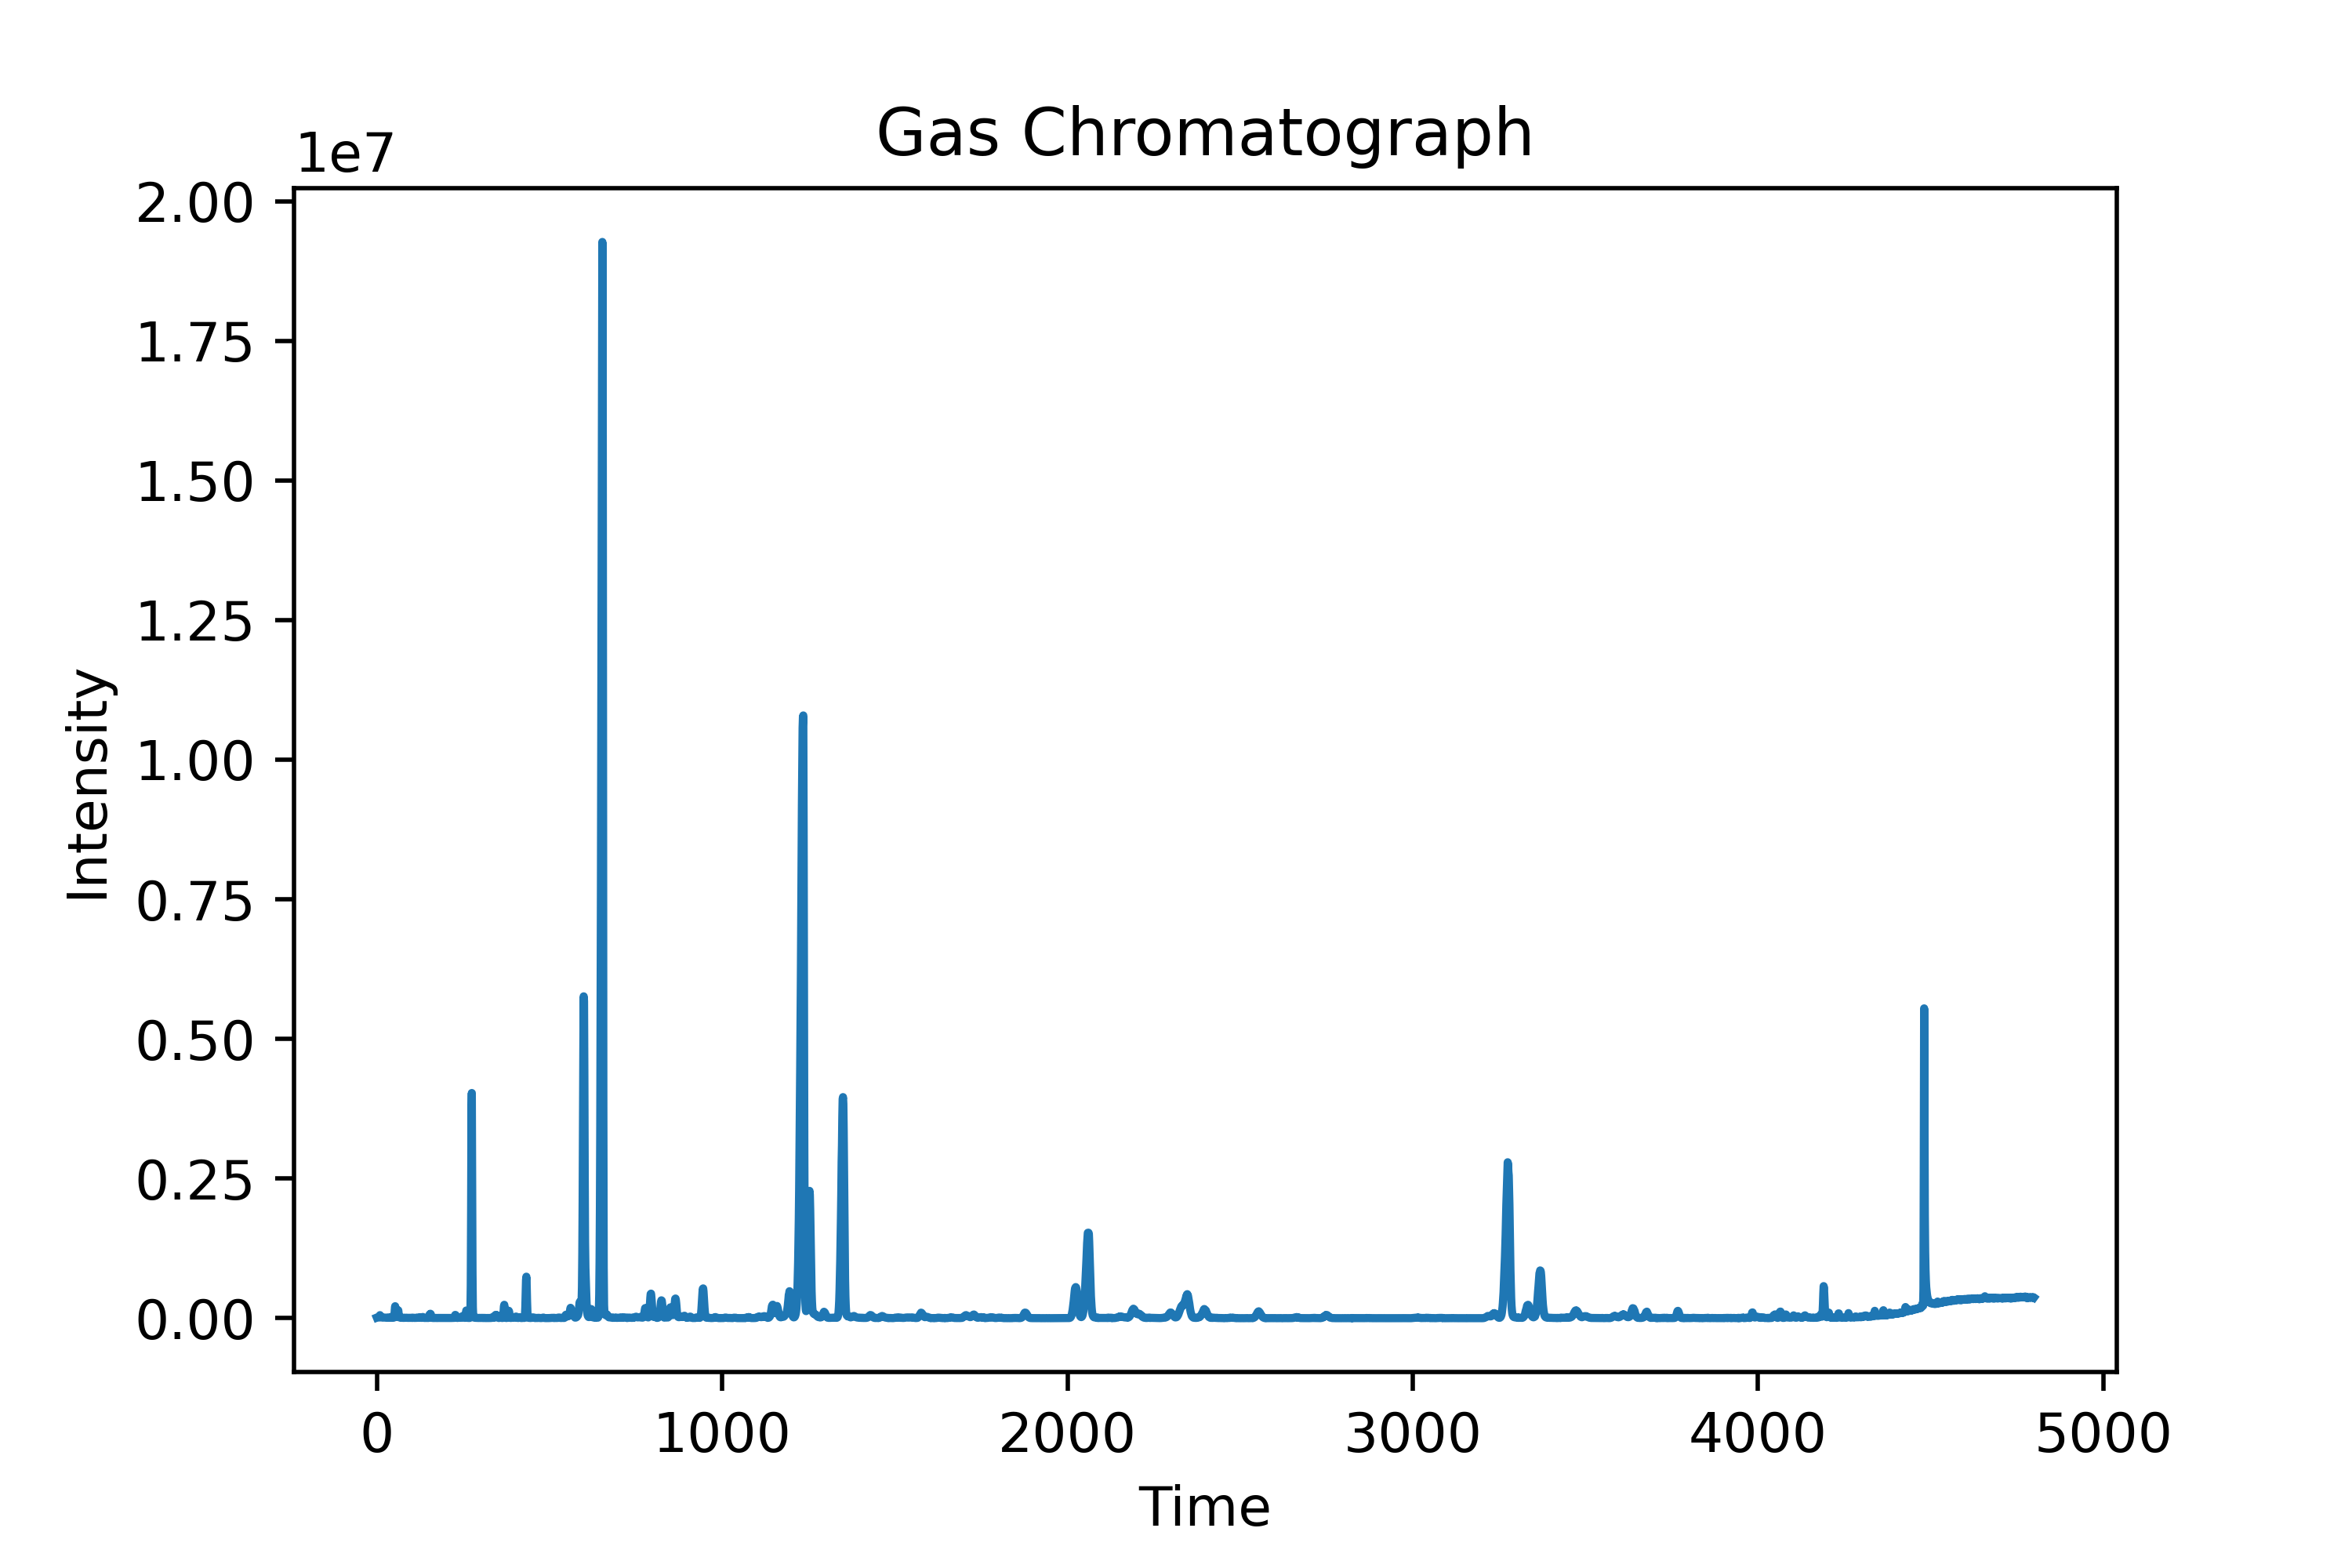
\includegraphics[width=0.6\textwidth]{chromatograph.png}
  
  \caption{Gas Chromatogram of Fatty Acid Methyl Esters from Snapper Skin}
  \label{fig:gas-chromatography} 
\end{figure}

\section{Data Preprocessing and Formation of Classification Problems}

The Y-data output from the Gas Chromatography analysis consists of many packets with variable intensities. 
In theory, they could be used as features to classify the different fish samples, but there were a large number of inconsistencies between packets in the different fish samples. 
An example, focusing on these inconsistencies for three different fish samples, is shown in Table \ref{tb:badRaw}. 
Although all three samples have three packets, their timestamps are different. 
For example, the timestamp of the first packet of Sample 1 is 51, while the timestamp of the first packet of Sample 2 is 50. 
In other words, the first packet of Sample 1 does not correspond to the first packet of Sample 2, and thus it does not make sense to directly apply a classification algorithm to the raw data. 
Initial experiments tried KNN (K=3), and the classification performance was only 67\%, which is quite low. 

\begin{table}[t]
	\centering
	\caption{Inconsistent Timestamps}
	\label{tb:badRaw}
\begin{tabular}{|l|c|c|c|}
	\hline
	& \multicolumn{3}{c|}{Timestamp} \\
	\cline{2-4}
	& Sample 1 & Sample 2 & Sample 3\\
	\hline 
	Packet 1 & 51 & 50 & 50 \\
	Packet 2 & 52 & 51 & 51\\
	Packet 3 & 53.05 & 53.1 & 53 \\
	\hline
\end{tabular}
\end{table}

Further investigation revealed that the main reason was due to the missing packets, caused by the absence of signal at the Gas Chromatography detector. 
For example, for Sample 1, the packet at the timestamp 50 is missed, and thus the first packet of Sample 1 is at 51. 
These missing packets are unavoidable for this dataset, therefore a method is needed to handle missing data. 
Preprocessing aligns the packets from all the samples.
Firstly, all unique timestamps are collected by analysing all the possible samples in the training set. 
For the example given in Table \ref{tb:badRaw}, the set of unique timestamps is \{50, 51, 52, 53, 53.05, 53.1\}. 
Thus, there should be six packets in total, while Table \ref{tb:badRaw} shows only three packets for each sample. 
Based on the timestamp set, the packets at \{50, 53, 53.1\} are missing for Sample 1. 
Once the missing packets are identified, these missing intensities need to be filled.

This work tried three different standard methods for missing values: filling 0, filling the average value, and filling the median value. 
The results show that filling 0 gives the most promising results with 83.57\% on KNN (K=3). 
The possible reason is that the missing packets have low intensities, which the detector might not be able to detect. 
Thus, the 0 value is quite close to the intensities of the missing packets. 
Therefore, the filling 0 method was chosen. 
The authors are aware that there are more complex methods for imputing missing values, but they are not the focus of the paper and will be left for future work \cite{tran2015multiple}.

The processing gives 4800 packets for each sample, which meant each sample had \textit{4800} features. 
The number of fish samples was 153. 
There is a class imbalance for the fish species dataset, where Blue cod is the majority class e.g., 68 samples are Blue Cod of the total 153 samples.
There are two classification tasks associated with the data:

\begin{itemize}
	\item To predict the fish species for each fish sample. There are four fish species: \textit{Snapper, Gurnard, Tarakihi}, and \textit{Blue cod}.
	\item To predict from which body part the fish sample is extracted. There are six body parts: \textit{Frame, Gonad, Head, Liver, Skin}, and \textit{Guts}.
\end{itemize} 

\section{Classification Performance}

The following section illustrates the classification performance on the fish species and body parts.

\subsection{Experiment Settings}

Firstly, since the number of samples is small, the experiment uses 10-fold cross-validation to conduct the experiments. 
For 10-fold cross-validation, the method divides the data into 10 folds such that the proportions of the classes in each fold are representative of the proportions in the whole dataset. 
Each fold plays the testing role, while the remaining 9 folds are combined to form a training set. 
A classification algorithm is then trained on the training set, and the obtained classifier is evaluated on the test set. 
Finally, 10 testing accuracies are obtained, and their mean value and standard deviation are given as the final classification performance. 
The experiment measures the balanced accuracy, so as not to bias results towards the majority class (i.e. Blue cod).

These experiments compare five well-known classifications: K Nearest Neighbours (KNN where K is set to 3), Naive Bayes (NB), Random Forest (RF), Decision Trees (DT), and Linear Support Vector Machines (SVM)  \cite{fix1989discriminatory,hand2001idiot,ho1995random,loh2011classification,cortes1995support}. 
The parameters are the default settings in \textit{scikit-learn} \cite{pedregosa2011scikit}.

\subsection{Results and Discussion}

\begin{table}[htb]
  \captionsetup{font=small,labelfont=small}
  \caption{
    Classification Accuracies
    }
  \centering
  \begin{tabular}{|l|l|l|l|l|}
    \hline
    Dataset                    & Method & 
    AvgTrain $\pm$ Std         & 
    % T                          &
    AveTest $\pm$ Std                      \\ % &
    % T                                     \\
    \hline
    Fish Species                    & 
    \begin{tabular}[c]{@{}l@{}}
      KNN          \\ % K-Nearest Neighbors
      RF           \\ % Random Forest
      DT           \\ % Decision Tree
      NB           \\ % Naive Bayes
      \textbf{SVM} \\ % Support Vector Machine
    \end{tabular} & 
    \begin{tabular}[c]{@{}l@{}}
      83.57 $\pm$ 1.80         \\ % KNN
      100.0 $\pm$ 0.00          \\ % RF
      100.0 $\pm$ 0.00          \\ % DT
      79.54 $\pm$ 1.60         \\ % NB
      \textbf{100.0 $\pm$ 0.00} \\ % SVM
    \end{tabular} & 
    \begin{tabular}[c]{@{}l@{}}
      74.88 $\pm$ 12.54          \\ % KNN
      85.65 $\pm$ 10.76          \\ % RF
      76.98 $\pm$ 13.12          \\ % DT
      75.27 $\pm$ 4.35           \\ % NB
      \textbf{98.33 $\pm$ 5.00 } \\ % SVM
    \end{tabular}             \\
    \hline
    Body Parts                       & 
    \begin{tabular}[c]{@{}l@{}}
      KNN          \\ % K-Nearest Neighbors
      RF           \\ % Random Forest
      DT           \\ % Decision Tree
      NB           \\ % Naive Bayes
      \textbf{SVM} \\ % Support Vector Machine
    \end{tabular} & 
    \begin{tabular}[c]{@{}l@{}}
      68.95 $\pm$ 3.49          \\ % KNN
      100.00 $\pm$ 0.00           \\ % RF
      100.00 $\pm$ 0.00           \\ % DT
      65.54 $\pm$ 2.69          \\ % NB
      \textbf{100.00 $\pm$ 0.00 } \\ % SVM
    \end{tabular} & 
    \begin{tabular}[c]{@{}l@{}}
      43.61 $\pm$ 13.48          \\ % KNN
      72.60 $\pm$ 16.15          \\ % RF
      60.14 $\pm$ 14.57          \\ % DT
      48.61 $\pm$ 12.19          \\ % NB
      \textbf{79.86 $\pm$ 8.52 } \\ % SVM
    \end{tabular}             \\
    \hline
  \end{tabular}
  \label{t:classification}
\end{table}

Table~\ref{t:classification} shows the results for KNN, RF, DT, NB, and SVM. 
Results are given for fish species (top), and fish part (bottom) datasets. 
The mean and standard deviation of balanced accuracy is given using the fish species and part datasets. 
For each dataset, the best accuracy is emphasized in bold. 

As can be seen from the table, RF, DT and SVM achieve 100\% training accuracies. 
However, on the test set, DT and RF do not achieve good classification performance. 
The main reason is that there is a small number of training samples. 
The trees built by DT and RF can perfectly fit the training data by creating large trees that remember all the possible training samples. 
Such trees do not generalise well on the test set, which is the overfitting problem in machine learning. 
KNN does not achieve good performance since it is a distance-based classification algorithm which suffers the most from the large number of features. 
Similar to KNN, NB does not achieve good performance since it assumes conditional independence between features that may not be true in the fish datasets. 
The SVM classifier outperforms the other classifiers on the test set, with 98.33\% and 79.86\% for fish species and body parts, respectively. 
The main reason is that SVM can handle a large number of features, so SVM is suitable to classify the fish data. 

Another essential point is that the classification accuracy on the fish species is always higher than the classification accuracy on the body parts. 
The results suggest that classifying body parts is a more challenging problem. 
A possible reason is that the tissue samples from different species may have very different chemical components. 
Meanwhile, the tissue samples from different body parts (but on the same fish species) may have similar chemical components. 
Future work will investigate more sophisticated mechanisms to improve the classification performance on classifying body parts. 

\begin{figure}[t]
	\centering
	\begin{subfigure}[b]{.49\linewidth}
		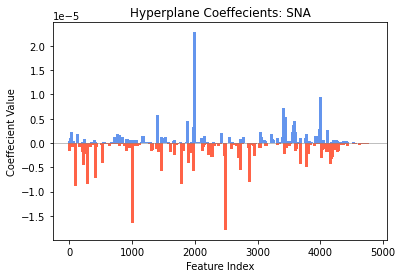
\includegraphics[width=\linewidth]{fish_hyperplane_sna.png}
		\caption{Snapper}\label{fig:hyperplane-sna}
	\end{subfigure}
	\begin{subfigure}[b]{.49\linewidth}
		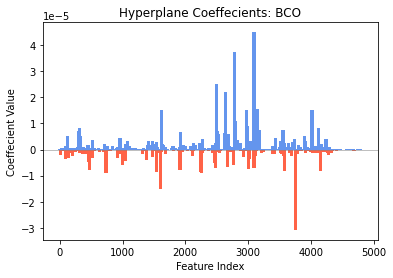
\includegraphics[width=\linewidth]{fish_hyperplane_bco.png}
		\caption{Blue cod}\label{fig:hyperplane-bco}
	\end{subfigure}
 
	\caption[SVM Coef]{
		SVM Hyperplane Coefficients
	}
	\label{fig:svm-hyperplane}
\end{figure}

\subsection{Interpret SVM models}

Achieving a high classification performance is great. 
However, in real-world applications, it is essential to analyse why the models work well.
This subsection analyzes the SVM models built to classify the fish species. 
The main idea of SVM is to build hyperplanes that separate different fish species. 
The hyperplane is represented by a weight vector in which each weight is associated with a feature. 
The larger the weight, the more important the corresponding feature. 
After an SVM classification algorithm is trained on the training set, an SVM classifier containing a learned weight vector is obtained. 
This section analyses the learned weight vector to examine the contribution of each packet/feature.

Figures \ref{fig:hyperplane-sna} and \ref{fig:hyperplane-bco} show the coefficients of hyperplanes to separate Snapper and Blue cod from other species, respectively. 
The horizontal axis is the feature index and the vertical axis is the coefficient value. 
The negative weights are in red and the positive weights are in blue. 
Gas Chromatography data is non-negative, so only negative weights push toward the negative class, therefore positive weights are expected values, and the negative values are not.
Note that when considering the feature importance, the absolute values of the weights should be considered, i.e., the longer the bar, the more important the corresponding features. 
Both figures demonstrate that most features have relatively small weights, which suggests not all the 4800 packets/features are needed to classify the fish data.  

\section{Feature Selection}

\subsection{Motivations}

As can be seen in the SVM models, it is not necessary to use all the 4800 packets/features to perform fish classification.
Therefore, the number of packets can be reduced while maintaining (or even improving) the classification performance.
In an overall automated classification system, it would be great to significantly reduce the number of packets.
Since then the system will not need to wait for a large number of packets to arrive at the end of the detector, hence significantly improving the system efficiency and throughput. 
The remaining question is which packets or features should be used. 
This question motivates us to conduct a further investigation using feature selection to select the most important packets/features. 

\subsection{Feature Selection Methods}

In a classification problem, the classification performance relies heavily on feature quality. 
However, in a large set of features as in the fish data, there are usually redundant or irrelevant features that blur useful information provided by the relevant features. 
Feature selection aims to select an informative subset of relevant features, which is expected to significantly reduce the number of features while maintaining (or even improving) the classification performance.
In a feature selection system, subset evaluation is an essential component that evaluates the quality of a feature subset. 
Based on the subset evaluation, the system can continuously improve the subset quality until a stopping criterion is met. 
The final feature subset is the output as the final solution. 

This section compares four common feature selection methods: 

\begin{itemize}
	\item $\boldsymbol{\chi^2}$ (chi-square) \cite{liu1995chi2} is a statistical measure that computes the independence of two variables $X$ and $Y$. The formula of $\chi^2$ is
	\begin{equation}
	\chi^2 = \sum_{k=1}^N \frac{(X_{k} - Y_{k})^2}{Y_{k}}
	\label{eq:chi}
	\end{equation}
	where $k$ is the index of the sample and $N$ is the number of samples. 
	In feature selection, $\chi^2$ can be used to measure the independence between a feature and a class label. 
	Since there is usually a high dependency between a relevant feature and a class label, the low $\chi^2$ value indicates that the features are more relevant. 
	Thus, the features can be ranked in ascending order and the top-ranked features can be selected. 
	\item \textbf{Minimum Redundancy and Maximum Relevance (mRMR)} \cite{ding2005minimum} uses mutual information to perform feature selection. 
	Mutual information between two variables $X$ and $Y$, i.e., $I(X; Y)$ calculates the dependency between two or more variables. 
	mRMR aims to select a feature subset such that the redundancy of the selected features is minimised and the relevance between the selected features and the class label is maximised. 
	Given a set of selected features $A$, the score of a feature $X_i$, i.e., $S_i$ is calculated by the following formula:
	\begin{equation}
	S_i = I(Y; X_i) - \frac{1}{|S|} \sum_{X_j \in A} I(X_i; X_j) 
	\label{eq:mrmr}
	\end{equation}  
    mRMR has many iterations where at each step mRMR will add the best feature based on Eq. (\ref{eq:mrmr}). 
    mRMR stops when a predefined number of features are selected. 
	\item \textbf{ReliefF} \cite{robnik2003theoretical} is a feature selection algorithm based on distance measures. 
	In ReliefF, a good feature should be able to well separate instances from different classes while the instances from the same class should not be far from each other. 
	The algorithm ranks all features based on the idea of nearest neighbours. 
	For a feature, if the distance between two nearest instances from \textit{different} classes (a miss) is large, the feature score is increased since the feature can well separate different classes. 
	On the other hand, if the distance between the two nearest instances from the \textit{same} class is large (a hit), the feature score is decreased. 
	In ReliefF, the higher the score, the more relevant the feature. Therefore, all features are ranked in descending order, and the top-ranked features are selected. 
	\item \textbf{Particle Swarm Optimisation (PSO) \cite{kennedy1995particle,7969325} for Wrapper Feature Selection} utilises the classification performance as the fitness function to achieve feature selection. 
	The main idea is to have a swarm of particles that can explore the feature subset space in parallel. 
	Each particle represents a feature subset. 
	The quality of each particle is the classification performance of the corresponding feature subset. 
	Since it is necessary to train a classification algorithm during the evaluation process, the classification algorithm is ``wrapped'' inside the PSO algorithm (that is why the algorithm is called Wrapper PSO). 
	In this work, a linear SVM is used as the wrapped classification algorithm since it achieves good classification performance. 
	Each particle records the best feature subset that it discovered so far (called personal best or $pbest$) and the best feature subset that is discovered by the whole swarm so far (called global best or $gbest$). 
	The particle then updates its position by moving towards the two best positions. 
	It is expected that the new subset at the new position will have better quality (i.e., higher classification performance) than the previous position. 
	An advantage of PSO is that the particle movement is stochastic. 
	Thus, the swarm can globally explore the feature subset search space, which is an essential point when dealing with a large and complex search space like feature selection. 
	Therefore, PSO has gained much attention from the feature selection community recently \cite{nguyen2020survey}.
\end{itemize}

Although there are other advanced and complicated feature selection algorithms \cite{li2017feature,zhang2020binary,alsahaf2022framework,alweshah2022coronavirus}, this work starts with the above four simple but well-known techniques. 
If the results are promising, future work will investigate extensions of these and/or other feature selection algorithms. 

\subsection{Experiment Settings}

Following the same setting in the classification part, this experiment uses 10-fold cross-validation to generate the training and test sets.  
For each method, the balanced classification accuracy is measured with a linear SVM classification algorithm \cite{sklearn2021feature}. 
For $\chi^2$, mRMR, and ReliefF, a hyperparameter for the number of selected features must be given. 
Therefore, the experiments measure the performance of the three algorithms on a wide range of the number of features: {50, 100, 150, ..., 4800} and the increment is 50. 
For PSO, the swarm size is set to 30 and the maximum number of iterations to 100.
An advantage of PSO is that it does not need to specify a hyperparameter for the number of selected features. 
Since PSO is a stochastic algorithm, it is run 30 independent times on each classification task to make a reliable comparison. 

\subsection{Feature Selection Performance on Fish Species Classification}

Figure~\ref{fig:fs-per-k-fish} shows the results for $\chi^2$ (chi2), ReliefF, mRMR and PSO on the fish species. 
The vertical axis is the classification accuracy and the horizontal axis is the number of selected features. 
As can be seen from the figures, the three algorithms $\chi^2$, mRMR, and ReliefF perform poorly when the number of selected features is small. 
The main reason is that when the number of selected features is small, many relevant features are not selected, and thus essential classification information is missed. 
Among the three algorithms, $\chi^2$ usually achieves the lowest classification performance since $\chi^2$ does not reduce the feature redundancy and does not consider the interactions between features.
ReliefF and mRMR achieve comparative performance. 
mRMR achieves its highest training and testing accuracies when the number of selected features is around 1500, which can be seen in Table \ref{tb:bestSpecies}. 

\begin{figure}[t]
  \centering
  \begin{subfigure}[b]{.45\linewidth}
    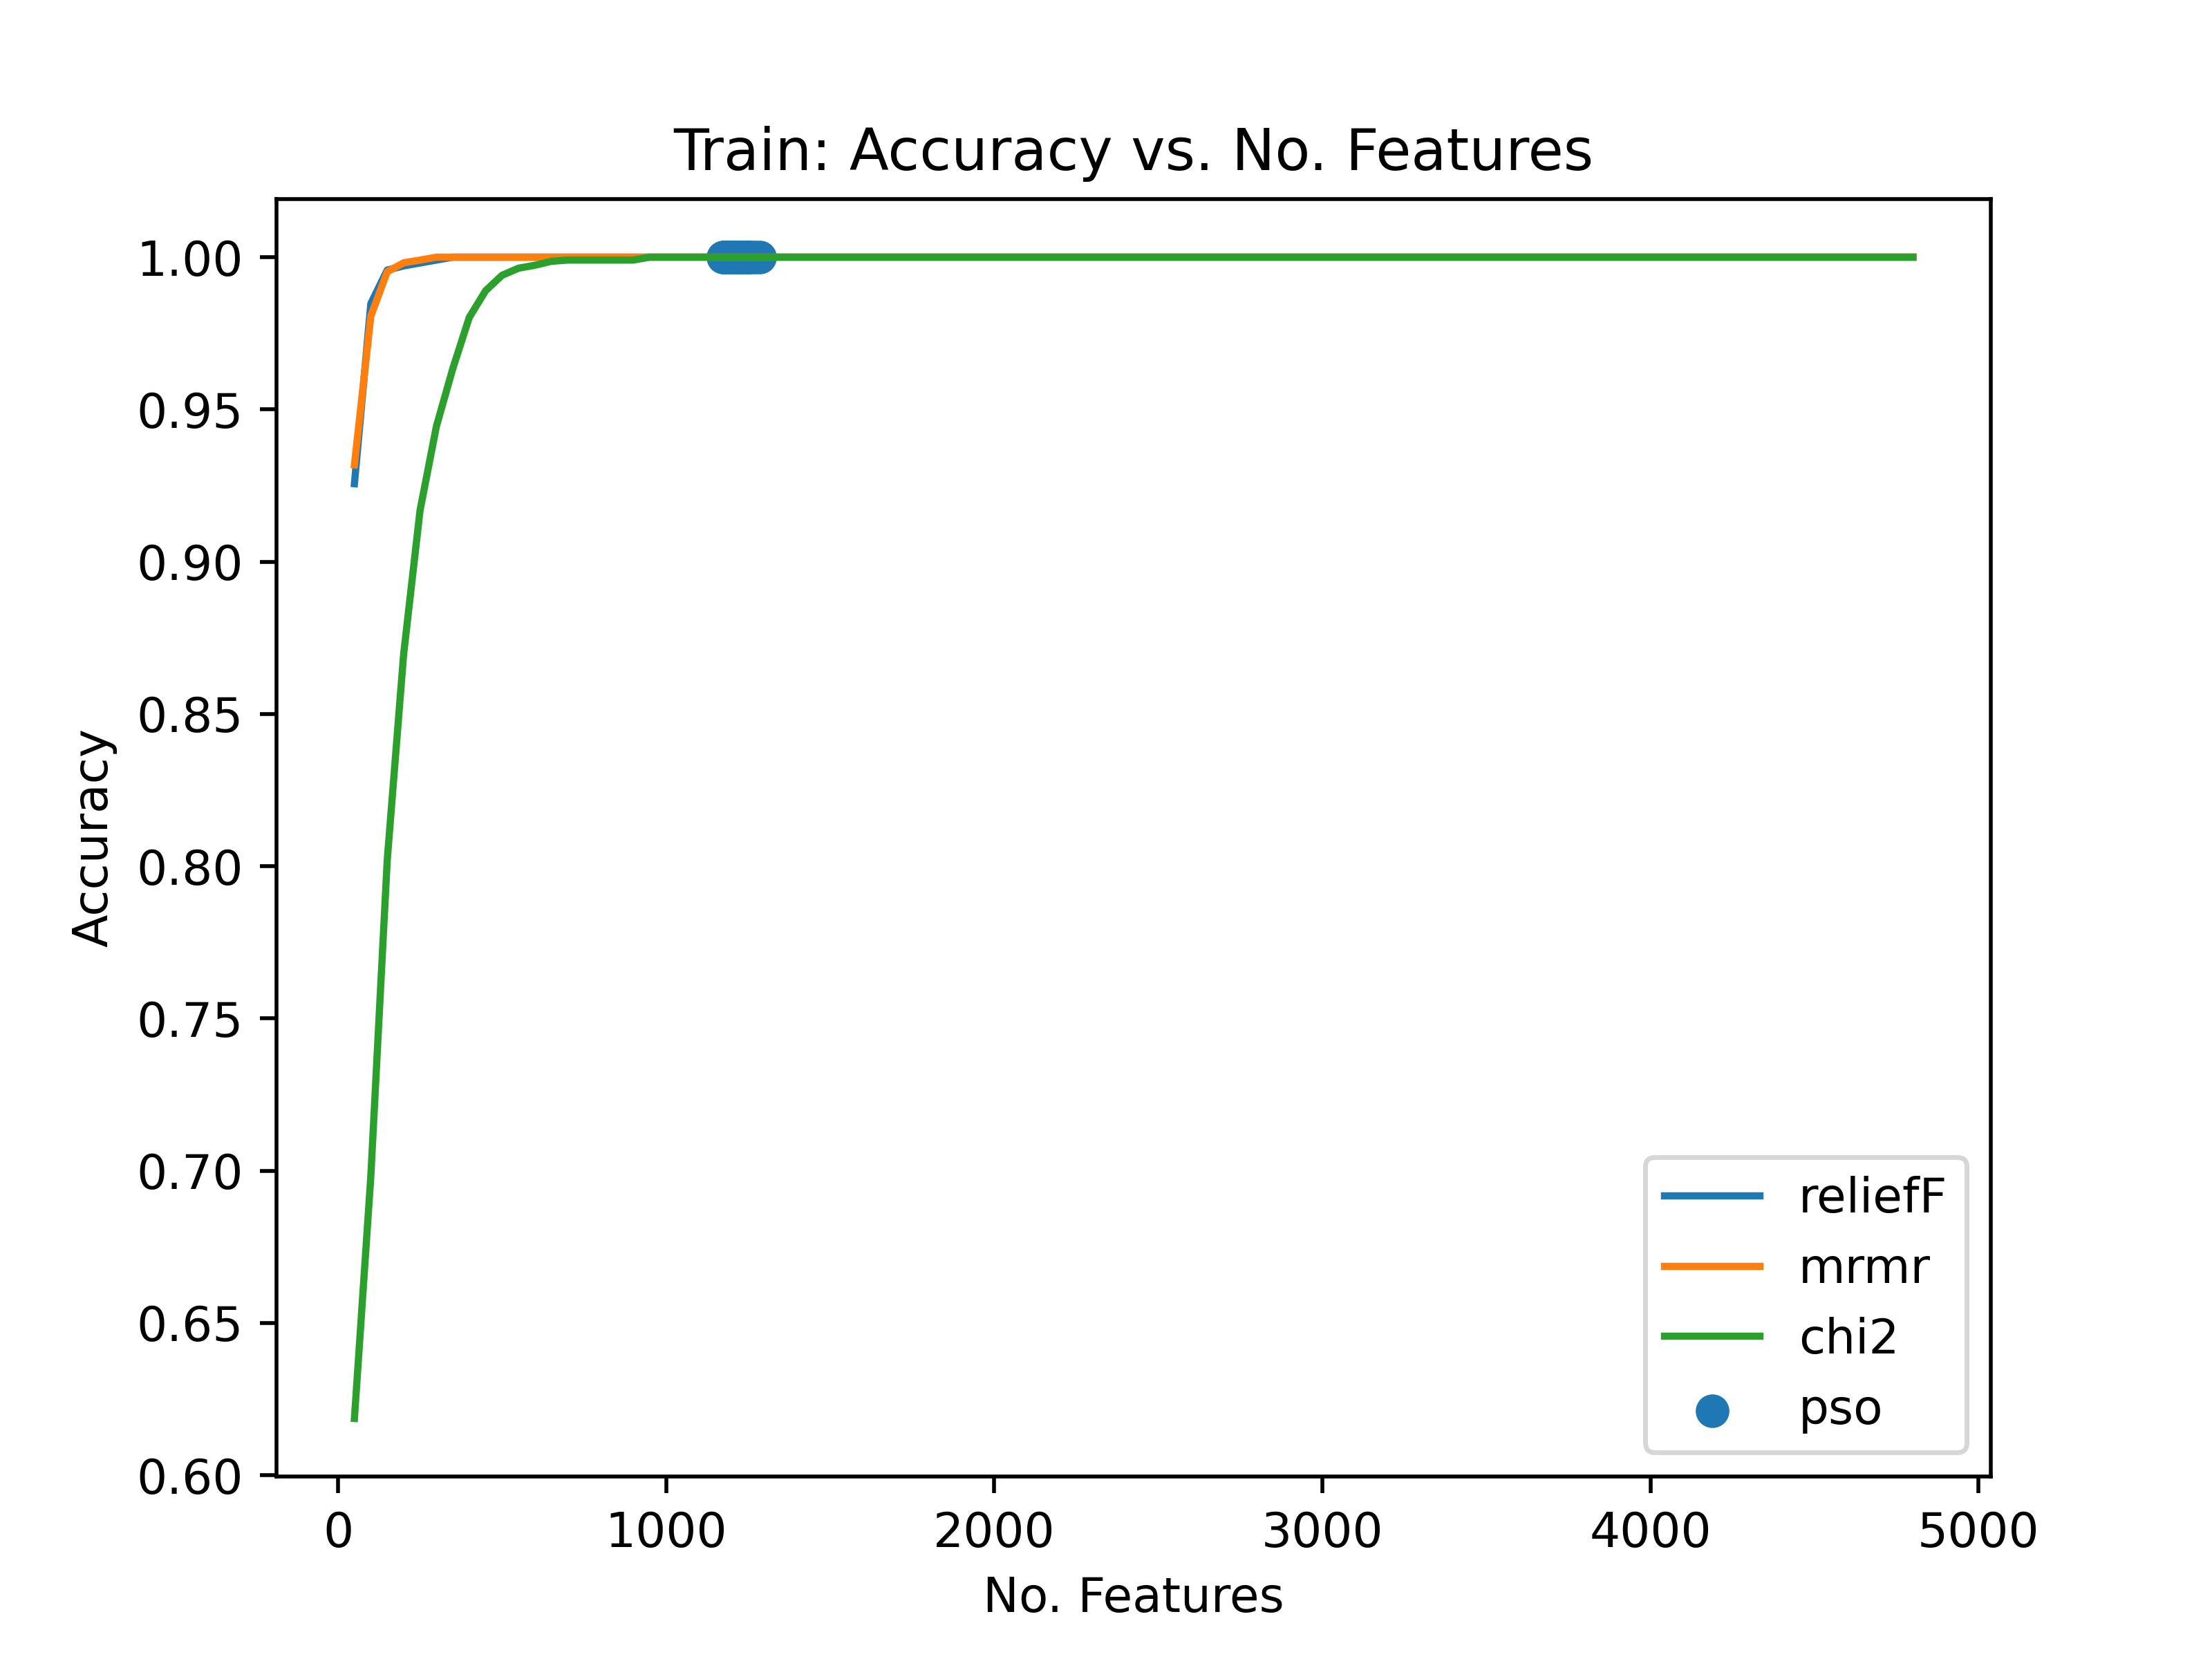
\includegraphics[width=\linewidth]{accuracy-features-fish-train.png}
    \caption{Species: Training set}\label{fig:fs-per-k-fish-train}
  \end{subfigure}
  \begin{subfigure}[b]{.45\linewidth}
    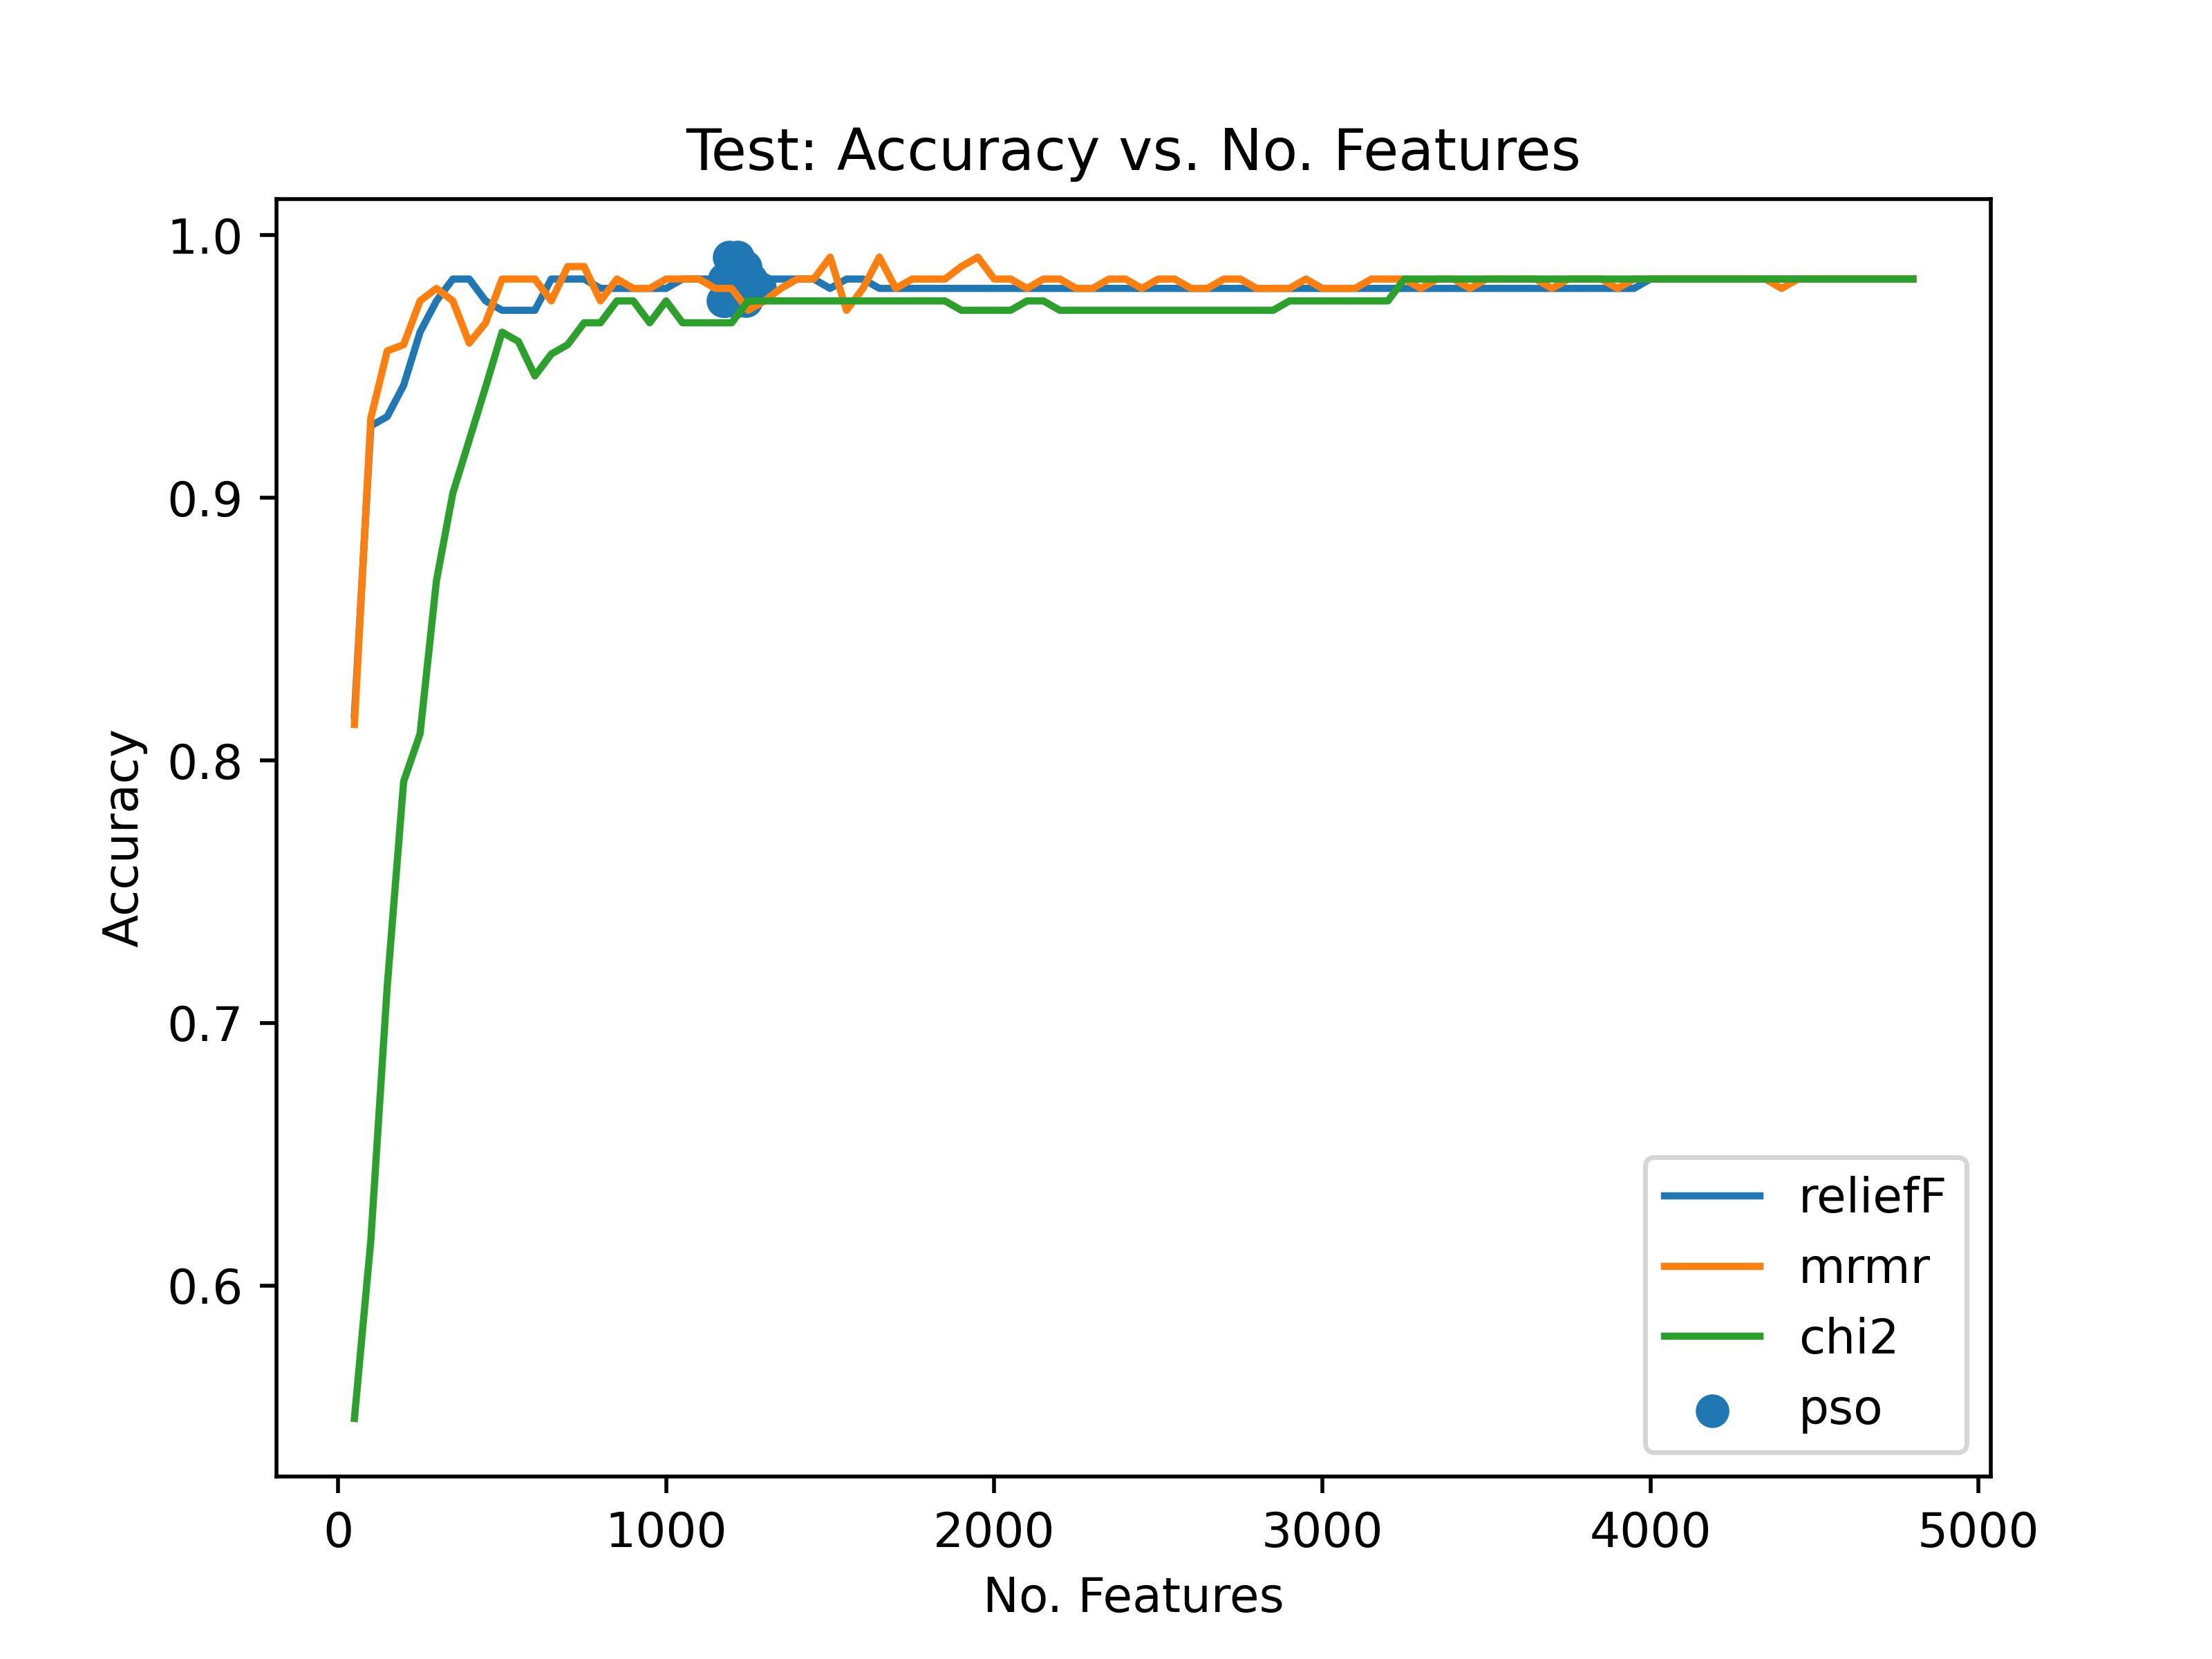
\includegraphics[width=\linewidth]{accuracy-features-fish-test.png}
    \caption{Species: Test set}\label{fig:fs-per-k-fish-test}
  \end{subfigure}
  \caption[Two numerical solutions]{
      Classification Accuracy of Fish Species on Different Numbers of Selected Features.
    }
  \label{fig:fs-per-k-fish}
\end{figure}

\begin{table}[t]
  \caption{
    Best accuracy on Fish Species.
    }
    \label{tb:bestSpecies}
  \centering
  \begin{tabular}{|l|c|c|c|}
    \hline
    Method & 
    Number of features &
    Training accuracy         & 
    Testing accuracy                     \\
    \hline
    \begin{tabular}[c]{@{}l@{}}
      ReliefF   \\        
      \textbf{mRMR}      \\     
      $\chi^2$      \\  
      \textbf{PSO}       \\
      Full      \\
    \end{tabular} & 
    \begin{tabular}[c]{@{}l@{}}
      359       \\ 
      \textbf{1500}      \\ 
      3250      \\ 
      \textbf{1192}      \\ 
      4800      \\
    \end{tabular} & 
    \begin{tabular}[c]{@{}l@{}}
      100.0     \\
      \textbf{100.0}     \\
      100.0     \\
      \textbf{100.0}      \\
      100.0      \\ 
    \end{tabular} & 
    \begin{tabular}[c]{@{}l@{}}
      98.33 \\
      \textbf{99.17} \\
      98.33 \\
      \textbf{99.17} \\
      98.33 \\ 
    \end{tabular}             \\
    \hline
  \end{tabular}
  \label{t:feature-selection}
\end{table}

As can be seen from the figure, most feature subsets evolved by PSO have from 1100 to 1500 features. 
The results indicate that PSO can automatically determine a good number of selected features, which cannot be achieved by the other three algorithms. 
As can be seen in Table \ref{tb:bestSpecies}, the highest classification performance of PSO is 99.17\% which is about 1\% higher than using all features. 
Meanwhile, PSO can remove 75\% features, which means the classification system can be four times faster given the number of required packets/features is reduced by four times. 

\subsection{Feature Selection Performance on Body Parts Classification}

\begin{figure}[t]
  \centering
  \begin{subfigure}[b]{.45\linewidth}
    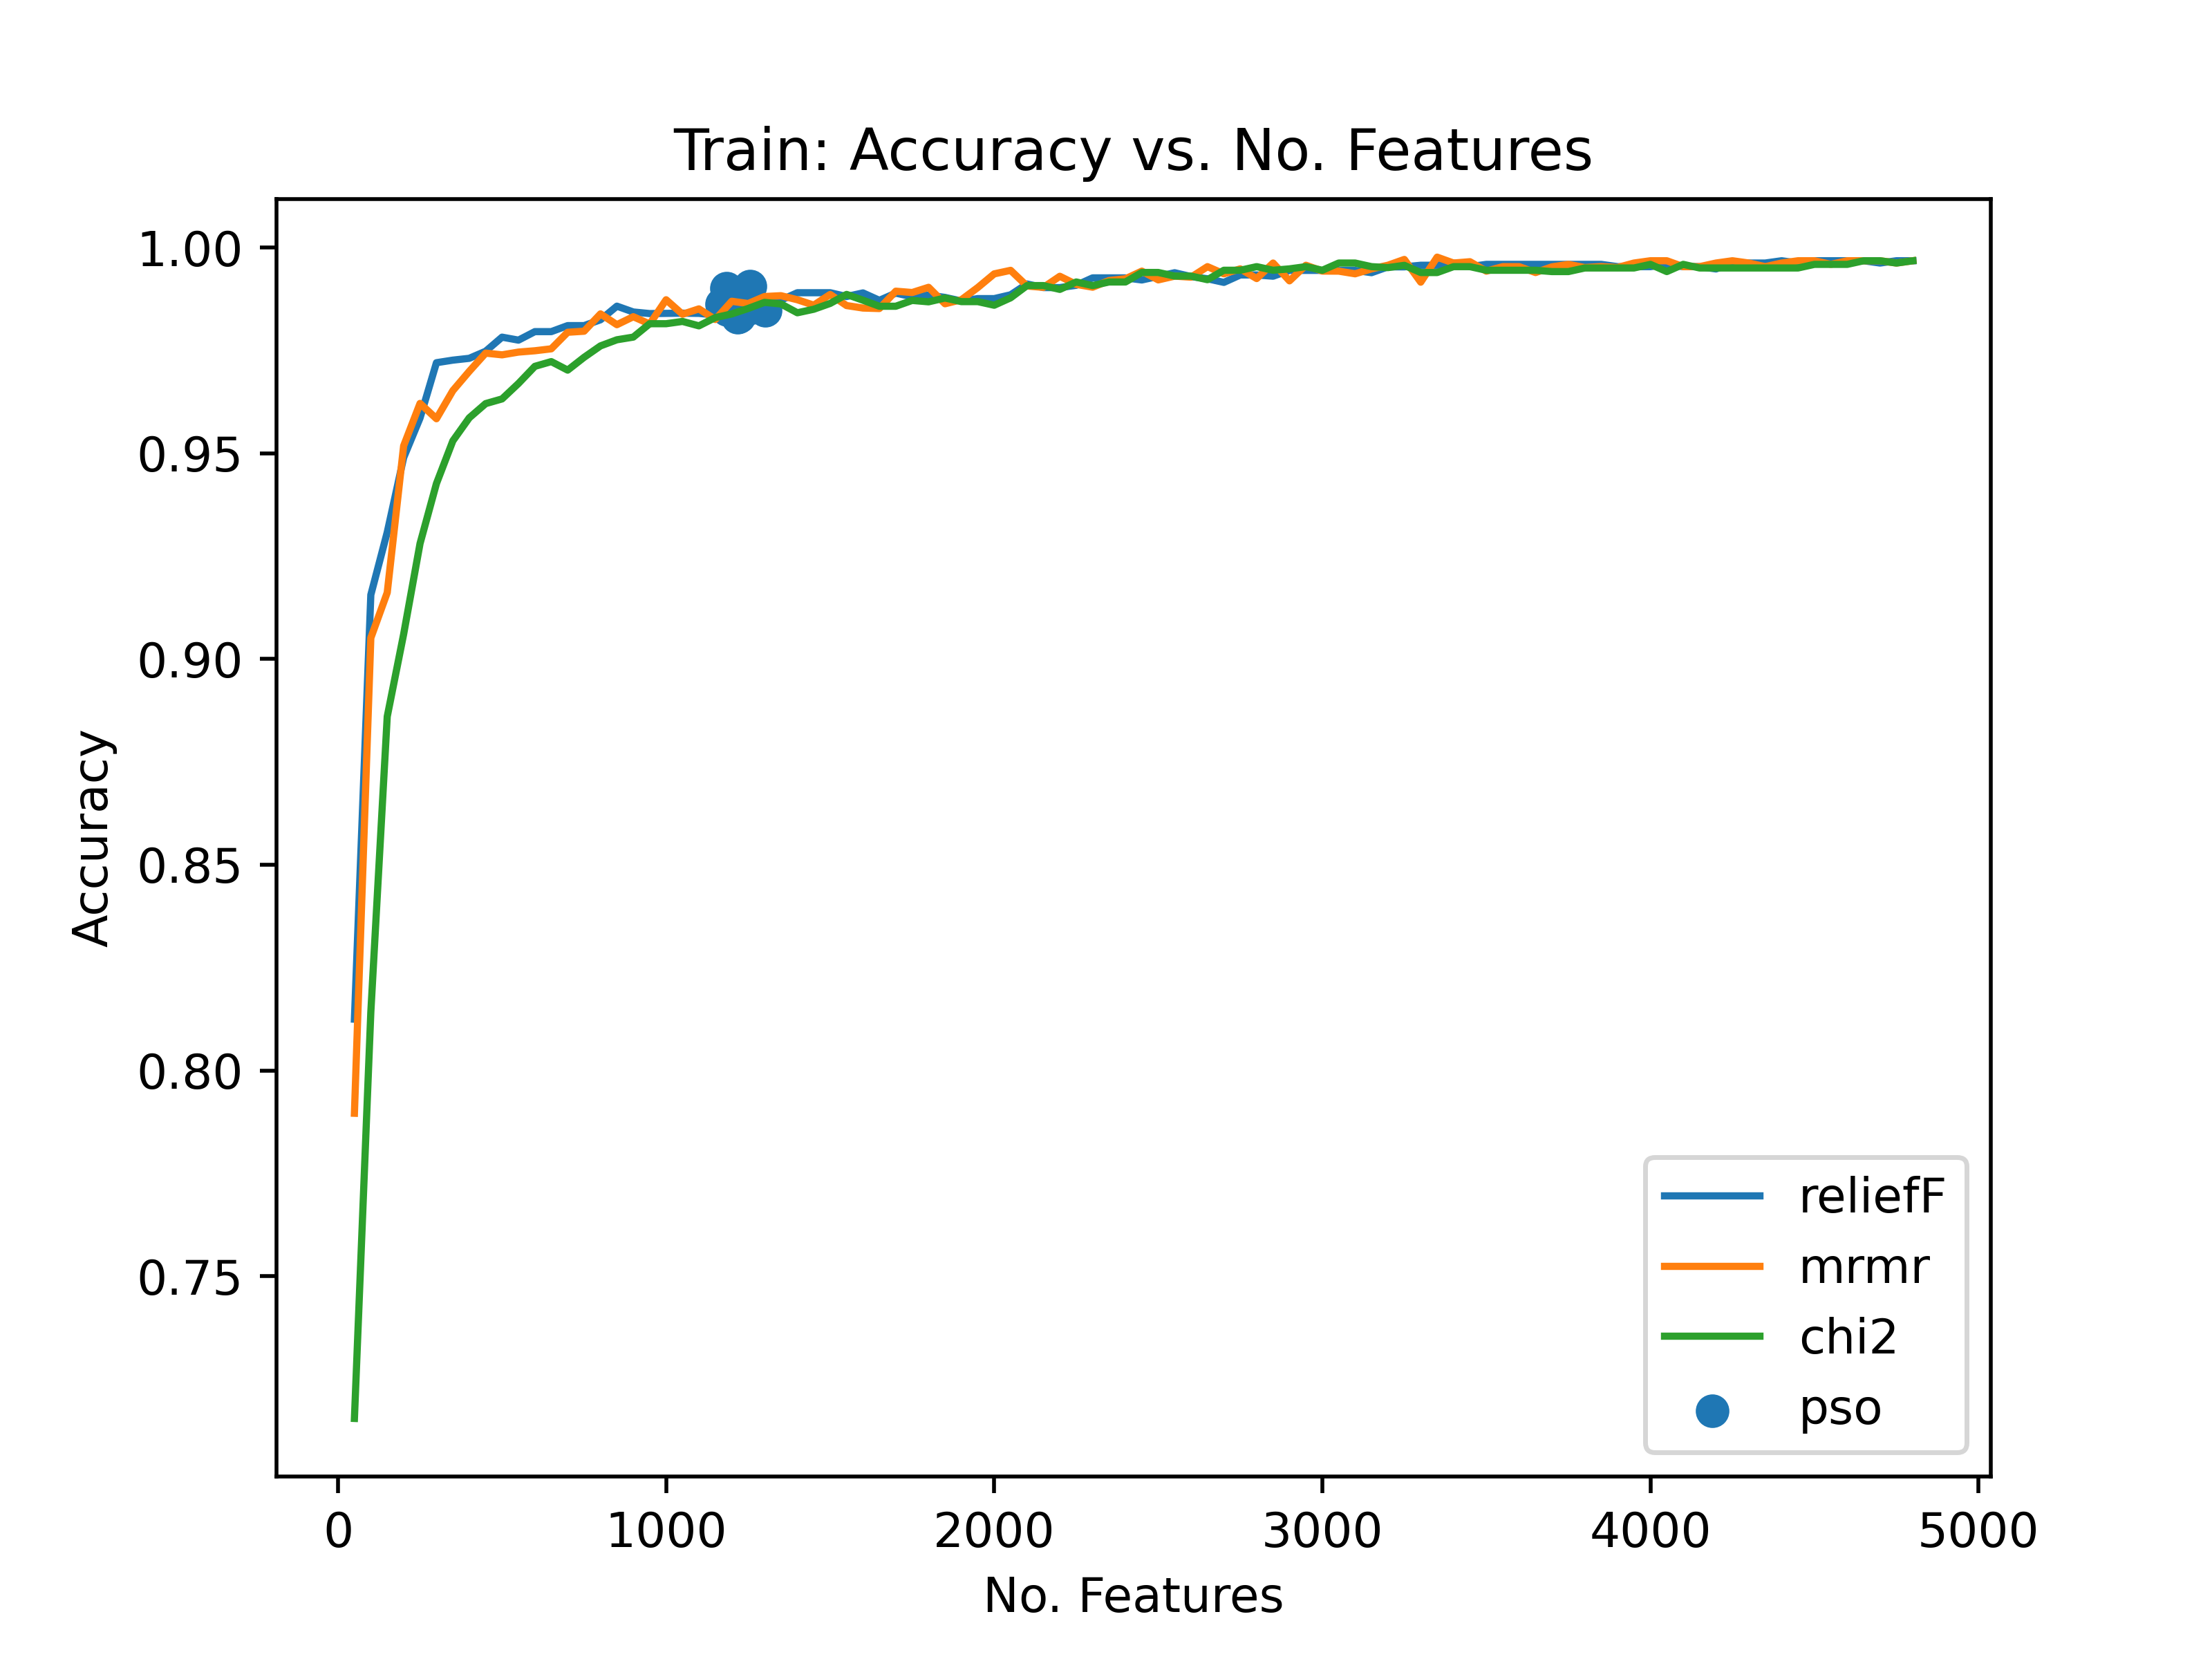
\includegraphics[width=\linewidth]{accuracy-features-part-train.png}
    \caption{Part: Training set}\label{fig:fs-per-k-part-part-train}
  \end{subfigure}
  \begin{subfigure}[b]{.45\linewidth}
    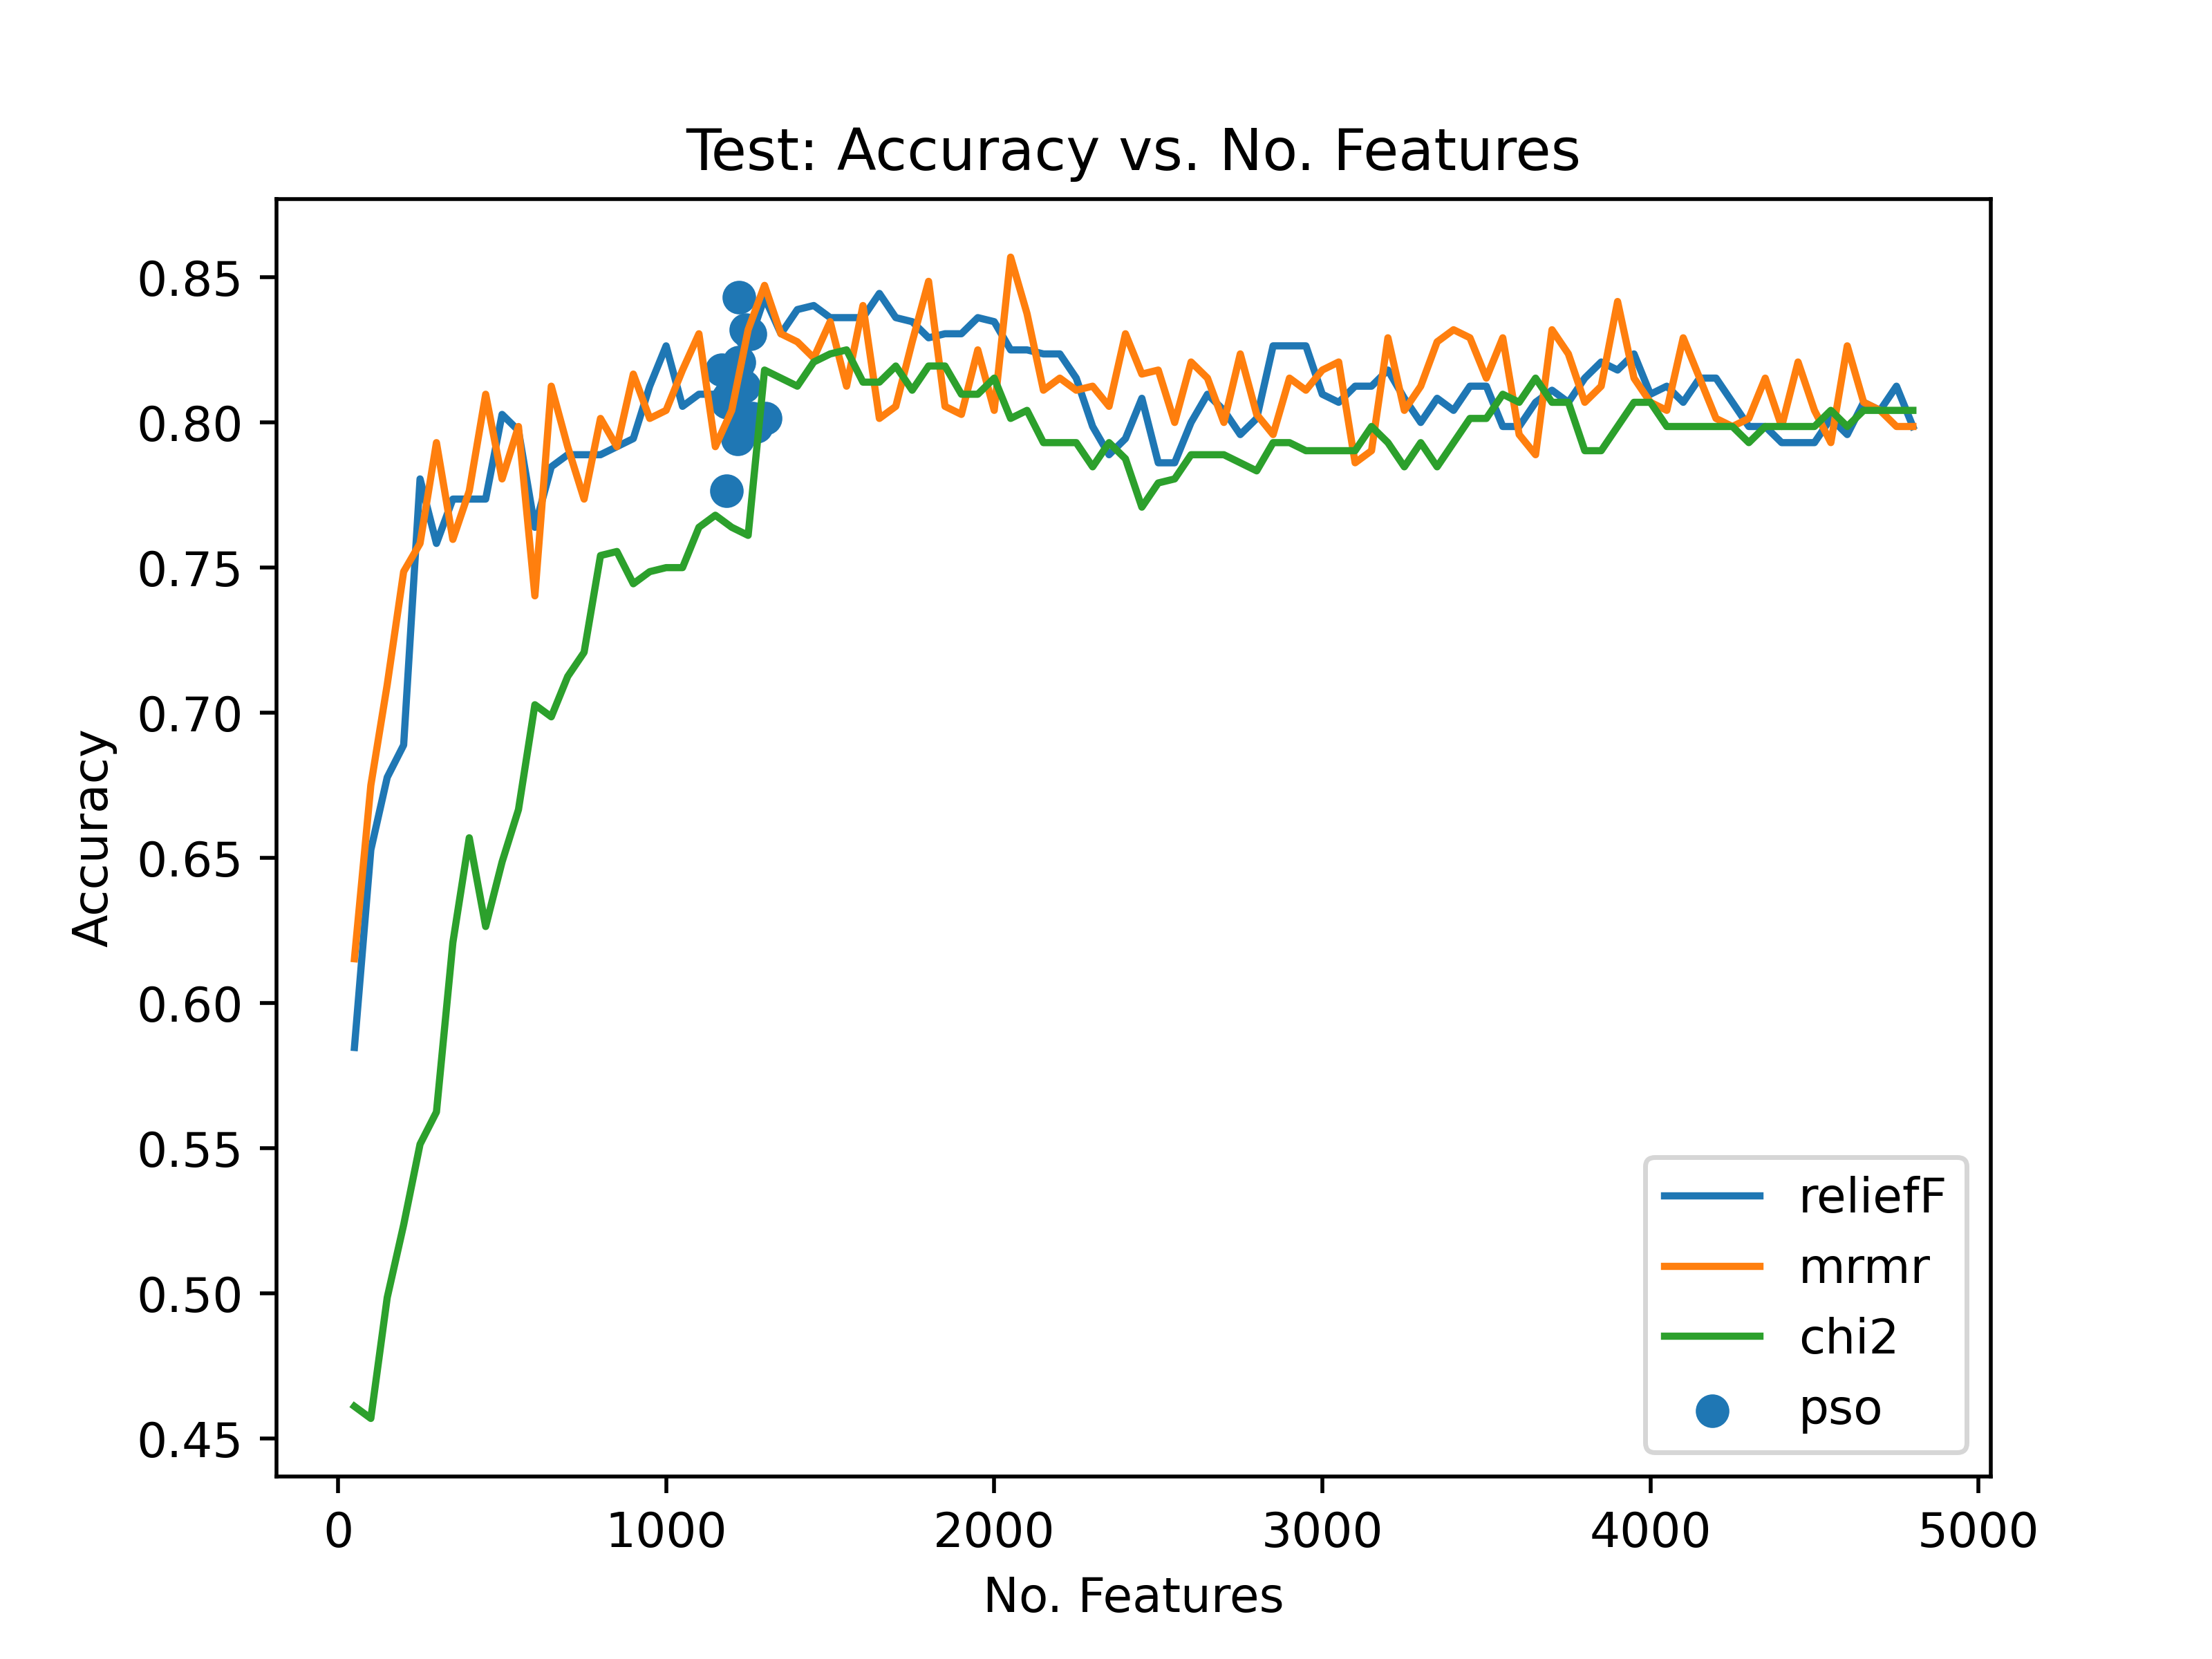
\includegraphics[width=\linewidth]{accuracy-features-part-test.png}
    \caption{Part: Test set}\label{fig:fs-per-k-part-part-test}
  \end{subfigure}
    \caption[Two numerical solutions]{
      Classification accuracy of Fish Body Parts on Different Numbers of Selected Features.
    }
  \label{fig:fs-per-k-part}
\end{figure}

Figure~\ref{fig:fs-per-k-part} shows the results for $\chi^2$, ReliefF, mRMR and PSO on the fish part dataset. 
As can be seen in Figure~\ref{fig:fs-per-k-part-part-train}, $\chi^2$, mRMR, and Relief-F witness a sharp improvement when the number of selected features is in the range [0, 500], which indicates that the 500 top-ranked features are essential to select. 
After that, the three approaches have a gradual incline, which peaks at 100\% where all the features are selected. 
On the other hand, PSO selected feature subsets with sizes ranging in [1200,1300]. 
Given the same classification performance, PSO usually selects a smaller number of features than the other three feature selection algorithms. 
The main reason is that PSO considers the interaction in the whole set of features, meanwhile, the other algorithms only consider the pair-wise interactions between feature pairs. 

\begin{table}[t]
  \caption{
    Best Accuracy on Fish Body Parts
    }
    \label{tb:bestBody}
  \centering
  \begin{tabular}{|l|c|c|c|}
    \hline
    Method & 
    Number of features &
    Training Accuracy        & 
    Testing Accuracy                   \\
    \hline
    \begin{tabular}[c]{@{}l@{}}
      ReliefF   \\        
      \textbf{mRMR}      \\     
      $\chi^2$      \\  
      PSO       \\
      Full      \\
    \end{tabular} & 
    \begin{tabular}[c]{@{}l@{}}
      1650       \\ 
      \textbf{1500}      \\ 
      1550      \\ 
      1223      \\ 
      4800      \\
    \end{tabular} & 
    \begin{tabular}[c]{@{}l@{}}
      100.0     \\
      \textbf{100.0}     \\
      100.0     \\
      100.0      \\
      100.0      \\ 
    \end{tabular} & 
    \begin{tabular}[c]{@{}l@{}}
      84.44 \\
      \textbf{86.94} \\
      82.50 \\
      84.31 \\
      79.86 \\ 
    \end{tabular}             \\
    \hline
  \end{tabular}
  \label{t:feature-selection}
\end{table}

Table \ref{tb:bestBody} illustrates the best accuracy for classifying fish body parts. 
As can be seen from the table, the best classification performance at 86.94\% is achieved with 1500 features selected by mRMR. 
Thus, feature selection can also improve 7\% accuracy over using all features. 
Meanwhile, the number of features is reduced by 2.5 times, which means the system can be 2.5 times faster. 
It should be noted that the testing performance of PSO is not as good as mRMR despite its superior training performance. 
The results indicate the potential overfitting of PSO on classifying body parts, which can be investigated more in the future.

\subsection{Summary}
\label{sec:results-feature-selection-discussion}

In general, feature selection can significantly reduce the number of required packets/features while the classification performance is mostly maintained. 
For classifying the fish species, 75\% of packets can be removed. 
For classifying the body parts, 60\% of packets can be removed. 
The significant reduction means that the overall classification system can be up to 4 times faster. 
It should be noted that classifying the body part is more challenging than classifying the fish species. 
That is why classifying the body parts requires more features. 
Last but not least, PSO can automatically determine a good number of selected features. 
In general, PSO achieves good classification performance, except for some signs of overfitting which can be investigated in future. 

\section{Conclusions and Future Work}

This paper has proposed an interpretable and effective classification process for fish oil analysis. 
Based on the results, it can be concluded that machine learning is a promising direction to improve the effectiveness and efficiency of the overall fish product system. 
In terms of accuracy, the proposed model can achieve high classification performance on classifying both fish species and body parts. 
However, fish species are easier to predict than body parts since there is more intra-class variation within fish species than there is a similarity between the same part from different fish. 
Among the considered classification algorithms, linear SVM achieves the best classification performance since it is suited to high-dimensional problems. 
Analysis of the SVM model demonstrates that not all packets are needed, and thus feature selection has been conducted to significantly reduce the number of packets and improve the classification performance. 

It is worth noting that the classification and feature selection methods presented in this paper could be extended to further improve performance. 
This is particularly useful for the lower-accuracy fish part dataset. 
A potential direction is to improve the classification performance by constructing more informative high-level features, also known as feature construction. 
In addition, a more sophisticated imputation method can be developed to fill the missing packets in the fish data.

% Please note that the first paragraph of a section or subsection is
% not indented. The first paragraph that follows a table, figure,
% equation etc. does not need an indent, either.

% Subsequent paragraphs, however, are indented.

% \subsubsection{Sample Heading (Third Level)} Only two levels of
% headings should be numbered. Lower level headings remain unnumbered;
% they are formatted as run-in headings.

% \paragraph{Sample Heading (Fourth Level)}
% The contribution should contain no more than four levels of
% headings. Table~\ref{tab1} gives a summary of all heading levels.

% \begin{table}
% \caption{Table captions should be placed above the
% tables.}\label{tab1}
% \begin{tabular}{|l|l|l|}
% \hline
% Heading level &  Example & Font size and style\\
% \hline
% Title (centered) &  {\Large\bfseries Lecture Notes} & 14 point, bold\\
% 1st-level heading &  {\large\bfseries 1 Introduction} & 12 point, bold\\
% 2nd-level heading & {\bfseries 2.1 Printing Area} & 10 point, bold\\
% 3rd-level heading & {\bfseries Run-in Heading in Bold.} Text follows & 10 point, bold\\
% 4th-level heading & {\itshape Lowest Level Heading.} Text follows & 10 point, italic\\
% \hline
% \end{tabular}
% \end{table}


% \noindent Displayed equations are centred and set on a separate
% line.
% \begin{equation}
% x + y = z
% \end{equation}
% Please try to avoid rasterized images for line-art diagrams and
% schemas. Whenever possible, use vector graphics instead (see
% Fig.~\ref{fig1}).

% \begin{figure}
% 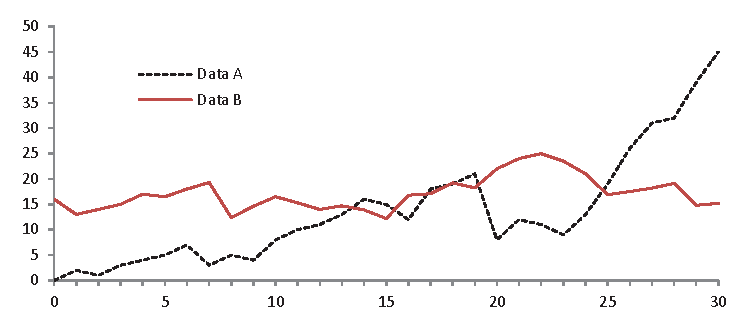
\includegraphics[width=\textwidth]{fig1.eps}
% \caption{A figure caption is always placed below the illustration.
% Please note that short captions are centred, while long ones are
% justified by the macro package automatically.} \label{fig1}
% \end{figure}

% \begin{theorem}
% This is a sampling theorem. The run-in heading is set in bold, while
% the following text appears in italics. Definitions, lemmas,
% propositions, and corollaries are styled the same way.
% \end{theorem}
%
% the environments 'definition', 'lemma', 'proposition', 'corollary',
% 'remark', and 'example' are defined in the LLNCS documentclass as well.
%
% \begin{proof}
% Proofs, examples, and remarks have the initial word in italics,
% while the following text appears in normal font.
% \end{proof}
% For citations of references, we prefer the use of square brackets
% and consecutive numbers. Citations using labels or the author/year
% convention are also acceptable. The following bibliography provides
% a sample reference list with entries for journal
% articles~\cite{ref_article1}, an LNCS chapter~\cite{ref_lncs1}, a
% book~\cite{ref_book1}, proceedings without editors~\cite{ref_proc1},
% and a homepage~\cite{ref_url1}. Multiple citations are grouped
% \cite{ref_article1,ref_lncs1,ref_book1},
% \cite{ref_article1,ref_book1,ref_proc1,ref_url1}.
%
% ---- Bibliography ----
%
% BibTeX users should specify bibliography style 'splncs04'.
% References will then be sorted and formatted in the correct style.
%
\bibliographystyle{splncs04}
% \bibliography{mybibliography}
\bibliography{refs}

\end{document}
